\chapter{Personal Preferences and Options}

There are some customizations that can be done on an individual basis. These options are available through the 
drop down menu on the top right side of the panel (see the highlighted red frame in the following figure).

\begin{figure}[H]
\centering
\fbox{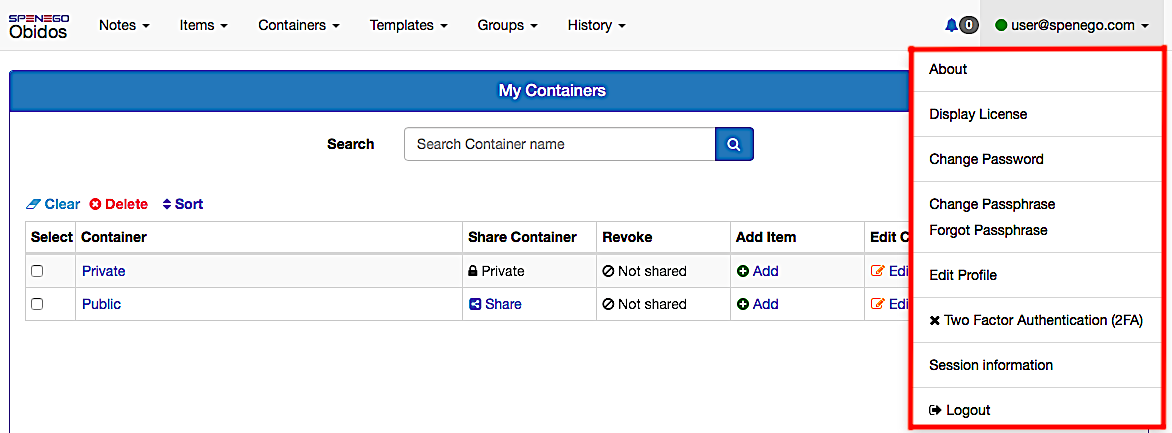
\includegraphics[scale=0.4]{user/Preferences.png}}
\caption{Preferences and Options menu}
\label{fig: Figure}
\end{figure}

\section{Display License}
The 'Display License' option shows your site license information for Obidos. 
The Open Source License has no expiration and supports any number of users. 
Standard and Enterprise Editions are annual subscription based. 
Once the license expires, users have 30 days of grace period
for using the software without interruption. During the 30-60 day period after license expiration, existing
entities can be viewed, but no new entities can be created. After 60 days of expiration, users will be
able to view only the license and their activity history; no other activities will be permissible.
List of all features available in each license edition is displayed in this screen.
\subsection{License Expiration}
30 days before the expiration of Obidos license, users will see warning message about license expiration.
This warning message will be displayed when the User logs into Obidos.
Once the license expires, users will have 30 days of grace period to use the software without disruption.
Between 30 days and 60 days after license expiration, users will not be able to create any new entities.
During this period, users can view their entities.
After 60 days of license expiration, they will not be able to use the software. A new license will need to be installed.
During the periods of disruption due to expired license, all user entities will remain intact in Obidos. 
Only with a valid license will users be able to use the software as usual.

\section{Change Password}
If the user account is local, then password can be changed using this option.

%\subsection{Changing Passphrase}
\section{Changing Passphrase}

If the User wants to change passphrase, it can be done through this option.
When the passphrase is reset, none of the existing entities owned by the User will be affected.

%\subsection{Forgotten Passphrase}
\section{Forgotten Passphrase}

\textcolor{red}{If the User forgets the passphrase, none of the stored Items can be retrieved.}
In this case, the User has two options. One is to reset the passphrase. The other is to create a new account
and start using Obidos from scratch.
If the User chooses to reset the passphrase, all the stored artifacts (Notes/Items/Containers) will be deleted and cannot be recovered. 
This is because Obidos will have to recreate a new key pair and overwrite the existing key pair.
Consequently, the previously stored artifacts (Notes/Items/Containers) cannot be recovered. Hence,
Obidos will delete those artifacts when the passphrase is reset.
An email with instructions for resetting the passphrase will be sent to the User. If the Administrator 
configured the account to use 2FA for passphrase reset, the User will be required to use 2FA as part of resetting
the passphrases.

If the User chooses to get a new account and start from scratch, all Notes/Items/Containers in the old account
will remain intact. If the User manages to remember/recover the passphrase for the old account even after creating a new account, 
it can be used as usual.
Note that it is not possible to merge the Notes/Items/Containers in two accounts.
Although, the User has the option to share Shareable Notes/Items/Containers from one account to the other and 
thus retrieve the contents of Shareable Notes/Items/Containers from one account; but this won't help in the case of Private Containers.


%\subsection{Edit Profile}
\section{Edit Profile}

The user can load a profile picture using the 'Upload new profile picture' button.
The profile picture can be deleted by using the 'Delete profile picture' button.

\begin{figure}[H]
\centering
\fbox{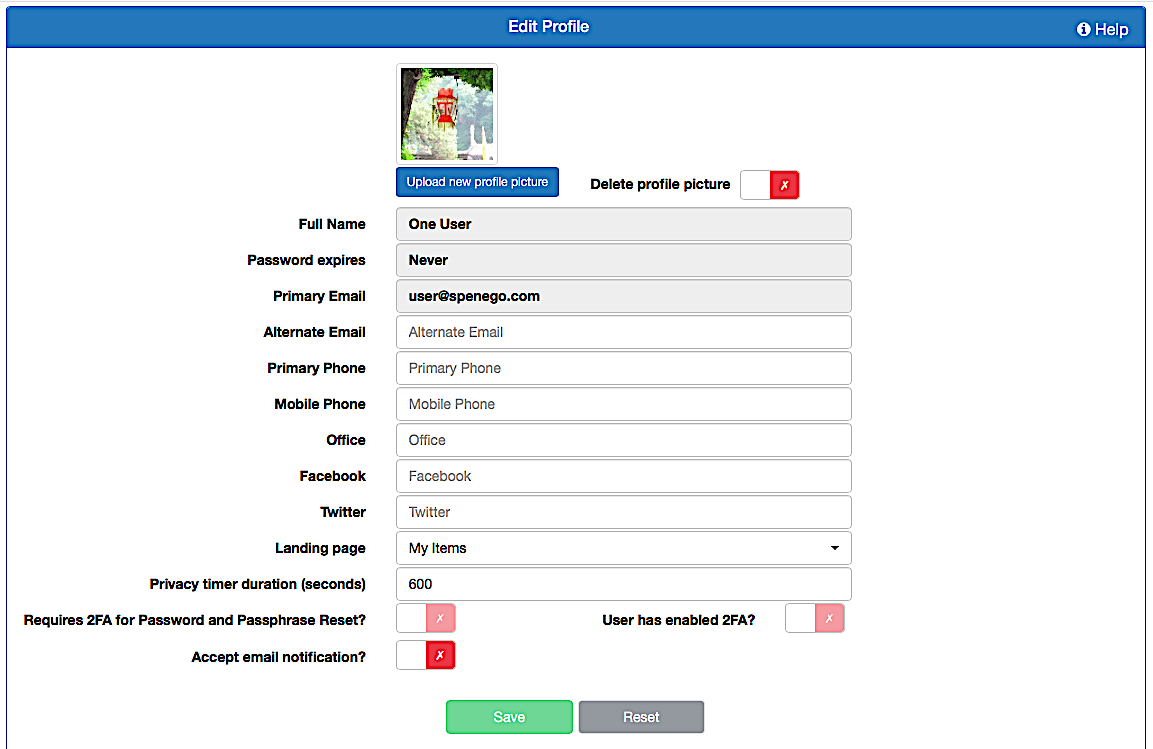
\includegraphics[scale=0.4]{user/User-profile.png}}
\caption{User Profile}
\label{fig: Figure}
\end{figure}

Alternate Email, Primary Phone, Mobile Phone, etc. are optional information.
\newline
\newline
'Landing Page' is the first page the User sees when logged in. The Landing page can be set to 'My Notes', 'My Items',
'My Containers', etc.
\newline
\newline
'Privacy timer duration' is the amount of time in seconds that an Item will be displayed for viewing.
The privacy timer starts as soon as an Item is displayed. At the end of the specified seconds, the Item will be hidden.
If you set the 'Privacy timer duration' to 0, then the timer will be off. 
\newline
\newline
The 2FA entries are only for information.
\newline
\newline
'Accept email notification?' flag is used by Obidos to screen email notifications. When a user shares an Item/Note/Container
with another user, the sender has the option to send an email notification to the recipient. 
Such notifications can be stopped by setting 'Accept email notification?' to x.

\section{Notifications}
Obidos has an internal notification system. This mechanism will notify the User when someone is sharing an entity 
or some user capabilities have been updated. Such notifications can be seen once the User logs into Obidos.

\begin{figure}[H]
\centering
\fbox{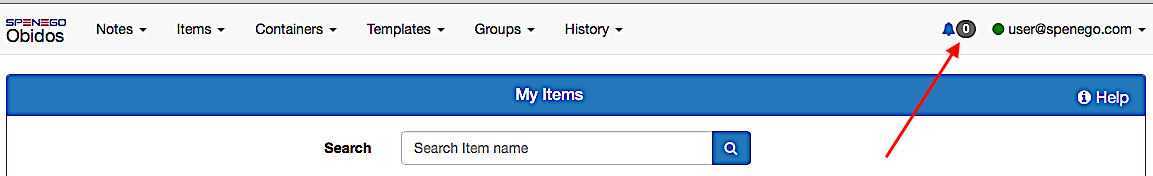
\includegraphics[scale=0.4]{user/Notifications-start.png}}
\caption{Notifications Status}
\label{fig: Figure}
\end{figure}

When notifications are present, the count will be displayed inside the red circle at the top right.
Clicking on the red circle will open up the 'Notification Messages' window.

\begin{figure}[H]
\centering
\fbox{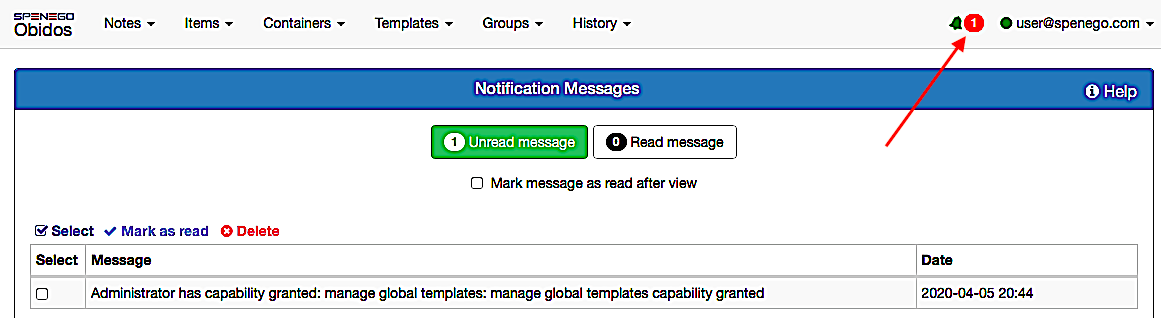
\includegraphics[scale=0.4]{user/Notifications-present.png}}
\caption{Notification Messages}
\label{fig: Figure}
\end{figure}

Some notifications are read only informational messages, while others are information links
that can be clicked on so that the entity referred in the message can be viewed.
If a notification is to be deleted, select the notification using the checkbox on the left and click on the
{\color{red}\faTimesCircle \ Delete} button.
